\documentclass[12pt,a4paper]{article}
\usepackage[utf8]{inputenc}
\usepackage[T2A]{fontenc}
\usepackage[russian]{babel}
\usepackage{geometry}
\usepackage{graphicx}
\usepackage{listings}
\usepackage{xcolor}
\usepackage{hyperref}
\usepackage{booktabs}
\usepackage{longtable}
\usepackage{amsmath}
\usepackage{float}

\geometry{
    left=30mm,
    right=15mm,
    top=20mm,
    bottom=20mm
}

\hypersetup{
    colorlinks=true,
    linkcolor=black,
    urlcolor=blue,
    citecolor=blue
}

\lstset{
    basicstyle=\ttfamily\small,
    breaklines=true,
    frame=single,
    backgroundcolor=\color{gray!10},
    keywordstyle=\color{blue},
    commentstyle=\color{green!60!black},
    stringstyle=\color{red},
    inputencoding=utf8,
    extendedchars=true
}

\begin{document}

% ==================== ТИТУЛЬНАЯ СТРАНИЦА ====================

\begin{titlepage}
    \centering
    \large

    \vspace*{1cm}

    \textbf{Московский авиационный институт}\\
    \textbf{(национальный исследовательский университет)}

    \vspace{1.5cm}

    Факультет информационных технологий и прикладной математики

    \vspace{0.5cm}

    Кафедра вычислительной математики и программирования

    \vspace{3cm}

    {\LARGE \textbf{Лабораторные работы по курсу}}\\
    \vspace{0.3cm}
    {\LARGE \textbf{<<Информационный поиск>>}}

    \vfill

    \begin{flushright}
        \begin{tabular}{rl}
            Студент: & З.\,Д.\,Брюханов \\
            Преподаватель: & А.\,А.\,Кухтичев \\
            Группа: & М8О-407Б-22 \\
            Дата: & 05.03.2026 \\
            Оценка: & \underline{\hspace{3cm}} \\
            Подпись: & \underline{\hspace{3cm}} \\
        \end{tabular}
    \end{flushright}

    \vspace{2cm}

    Москва, 2026
\end{titlepage}

\newpage

% ==================== ЛР 1 ====================

\section{Добыча корпуса документов}

\subsection{Цель работы}

Подготовить корпус документов для дальнейшего использования в задачах информационного поиска: выбрать источники, скачать данные, выделить текстовое содержимое и получить статистику.

\subsection{Источники данных}

Для формирования корпуса были выбраны два источника, объединённые тематикой <<мобильная разработка>>:

\begin{enumerate}
    \item \textbf{Habr.com} --- IT-платформа, хабы <<Мобильная разработка>>, <<Разработка под Android>>, <<Разработка под iOS>>. Статьи содержат технический текст на русском языке с вкраплениями английских терминов и фрагментов кода.

    \item \textbf{Wikipedia (ru)} --- русскоязычная Википедия, категории <<Мобильное программное обеспечение>>, <<Программное обеспечение для Android>>, <<Программное обеспечение для iOS>>. Энциклопедический стиль, структурированный текст, густая сеть внутренних ссылок.
\end{enumerate}

Выбор именно двух разнородных источников позволяет охватить и профессиональный (блоговый), и энциклопедический стиль изложения, что делает корпус более представительным.

\subsection{Характеристика документов}

Формат данных~--- HTML5 в кодировке UTF-8. Основной контент размещён в тегах \texttt{<p>}, \texttt{<h1>}--\texttt{<h6>}, списках \texttt{<ul>}/\texttt{<ol>}. На Habr часто встречаются блоки кода (\texttt{<pre><code>}), на Wikipedia~--- внутренние ссылки, сноски и таблицы.

Мета-информация присутствует в тегах \texttt{<meta>} (описание, ключевые слова), а также в разметке Open Graph (\texttt{og:title}, \texttt{og:description}).

\subsection{Выделение текста}

Очистка HTML выполняется библиотекой BeautifulSoup4 (Python): удаляются теги \texttt{<script>}, \texttt{<style>}, \texttt{<nav>}, \texttt{<footer>}, \texttt{<header>}, \texttt{<aside>}, \texttt{<noscript>}, после чего извлекается текстовое содержимое.

\subsection{Существующие поисковики}

Для проверки доступности документов использовались:
\begin{itemize}
    \item Встроенный поиск Habr (\texttt{habr.com/ru/search}).
    \item Поиск Google с оператором \texttt{site:}: \texttt{site:habr.com "flutter разработка"}.
    \item Встроенный поиск Википедии.
\end{itemize}

\textbf{Пример запроса:} \texttt{site:habr.com "android kotlin coroutines"}.

\textit{Результат:} Google находит релевантные статьи, однако в выдачу попадают страницы профилей пользователей, комментарии и дубликаты. Кроме того, невозможно выполнить булев запрос с оператором NOT по ограниченному подмножеству документов.

\textbf{Пример запроса:} \texttt{site:ru.wikipedia.org "мобильное приложение"}.

\textit{Результат:} Найдена основная статья и связанные страницы, но в выдачу попадают служебные страницы (<<Обсуждение:>>, <<Шаблон:>>).

\subsection{Статистика корпуса}

\begin{table}[h]
\centering
\begin{tabular}{@{}ll@{}}
\toprule
\textbf{Параметр} & \textbf{Значение} \\ \midrule
Количество документов & 30\,000 \\
Общий размер сырых данных (HTML) & 6.84 ГБ (7\,340\,032\,000 байт) \\
Общий размер чистого текста & 2.18 ГБ (2\,340\,716\,544 байт) \\
Средний размер сырого документа & 238.9 КБ \\
Средний объём текста в документе & 76.2 КБ \\
Доля полезного текста & 31.9\% \\ \bottomrule
\end{tabular}
\caption{Характеристики корпуса документов}
\end{table}

\subsection{Вывод}

Выбранные источники удовлетворяют требованиям: тематическая однородность (мобильная разработка), достаточный объём (30\,000 документов), наличие внешних поисковиков для проверки. Доля полезного текста составляет около 32\%, остальное~--- HTML-разметка, скрипты и стили, которые фильтруются при предобработке.

\newpage

% ==================== ЛР 2 ====================

\section{Поисковый робот}

\subsection{Цель работы}

Разработать краулер, который обходит веб-страницы по ссылкам, скачивает HTML и сохраняет в базу данных. Робот должен поддерживать возобновление работы после остановки.

\subsection{Метод решения}

Краулер реализован на Python. В качестве хранилища выбрана СУБД SQLite~--- весь корпус хранится в одном файле \texttt{crawler\_data.db}, что упрощает перенос и дальнейшую обработку на C++.

Конфигурация задаётся в файле \texttt{config.yaml}:

\begin{lstlisting}[language=yaml]
db:
  path: "crawler_data.db"
logic:
  request_delay: 0.15
  max_docs: 30000
  seed_urls:
    - "https://habr.com/ru/hubs/mobile_dev/articles/"
    - "https://habr.com/ru/hubs/android_dev/articles/"
    - "https://habr.com/ru/hubs/ios_dev/articles/"
    - "https://ru.wikipedia.org/wiki/..."
  allowed_domains:
    - "habr.com"
    - "ru.wikipedia.org"
\end{lstlisting}

\subsection{Архитектура}

Робот работает в режиме BFS (обход в ширину). Состояние хранится в двух таблицах SQLite:

\begin{itemize}
    \item \textbf{\texttt{pages}}~--- скачанные документы (id, url, source\_name, html\_content, fetched\_at).
    \item \textbf{\texttt{crawl\_queue}}~--- очередь URL со статусами: \texttt{waiting} $\to$ \texttt{active} $\to$ \texttt{done}.
\end{itemize}

При запуске робот проверяет состояние очереди и продолжает с того URL, на котором остановился. При повторном запуске уже скачанные документы не перекачиваются.

\subsection{Фильтрация URL}

Отсекаются ссылки на изображения (\texttt{.jpg}, \texttt{.png}, \texttt{.svg}), PDF, архивы, а также служебные страницы Wikipedia (\texttt{Special:}, \texttt{Служебная:}, \texttt{Обсуждение:}, \texttt{Файл:}, \texttt{Шаблон:}) и ссылки с параметрами редактирования (\texttt{action=edit}).

\subsection{Журнал выполнения}

В процессе реализации возникли проблемы:

\begin{enumerate}
    \item \textbf{Ловушки ссылок}~--- бесконечные ссылки на календари и служебные страницы Wikipedia. Решено расширением списка фильтров URL.

    \item \textbf{Блокировка запросов (HTTP 429/403)}. Решено добавлением задержки между запросами (\texttt{request\_delay: 0.15}) и корректного User-Agent.

    \item \textbf{Таймауты}. Некоторые страницы отвечают медленно. Установлен таймаут 10 секунд на запрос, при ошибке URL пропускается.
\end{enumerate}

\subsection{Тестирование}

\begin{longtable}{@{}clp{5cm}p{5cm}@{}}
\toprule
\textbf{\textnumero} & \textbf{Сценарий} & \textbf{Ожидание} & \textbf{Результат} \\ \midrule
\endfirsthead
\toprule
\textbf{\textnumero} & \textbf{Сценарий} & \textbf{Ожидание} & \textbf{Результат} \\ \midrule
\endhead
1 & Первый запуск & БД создана, данные начали поступать & Успешно \\
2 & Фильтрация & Ссылки на .jpg, Special: не попадают в очередь & Успешно \\
3 & Возобновление & После Ctrl+C и повторного запуска робот продолжает & Успешно \\
4 & Ошибка 404 & Страница пропускается, робот продолжает & Успешно \\ \bottomrule
\caption{Результаты тестирования краулера}
\end{longtable}

\subsection{Вывод}

Краулер успешно собирает корпус из двух источников с возможностью остановки и возобновления. SQLite в качестве хранилища обеспечивает надёжность (ACID) и удобство доступа из C++ на этапе индексации. Задержка между запросами и фильтрация URL предотвращают блокировки и ловушки.

\newpage

% ==================== ЛР 3 ====================

\section{Токенизация}

\subsection{Цель работы}

Реализовать алгоритм разбиения текста HTML-документов на токены (слова) и получить статистические характеристики процесса.

\subsection{Правила токенизации}

Токенизация реализована на C++ в файле \texttt{tokenizer.cpp}. Алгоритм выполняет однопроходную обработку:

\begin{enumerate}
    \item \textbf{Удаление HTML-тегов}: всё между \texttt{<} и \texttt{>} заменяется на пробел, чтобы не склеивались соседние слова.

    \item \textbf{Набор разделителей}: пробельные символы (ASCII $\leq$ 32), знаки препинания (\texttt{. , ! ? : ; " ' ( ) [ ] \{ \} < > / \textbackslash{} | - + = \# @ * \~{} ` \^{}}).

    \item \textbf{Нормализация}: латинские символы приводятся к нижнему регистру (A--Z $\to$ a--z). Кириллица передаётся как есть (UTF-8, без преобразования регистра в текущей реализации).

    \item \textbf{Формирование токена}: любая непрерывная последовательность символов, не являющихся разделителями.
\end{enumerate}

\subsection{Достоинства и недостатки}

\textbf{Достоинства:}
\begin{itemize}
    \item Линейная сложность $O(N)$~--- один проход по тексту без возвратов.
    \item Высокая скорость за счёт отсутствия регулярных выражений.
    \item Нормализация регистра уменьшает размер словаря.
\end{itemize}

\textbf{Недостатки:}
\begin{itemize}
    \item Технические термины (\texttt{C++}, \texttt{C\#}) распадаются на отдельные символы, так как \texttt{+} и \texttt{\#} считаются разделителями.
    \item URL-адреса, оставшиеся в тексте, порождают мусорные токены.
    \item Кириллический регистр не нормализуется~--- <<Андроид>> и <<андроид>> считаются разными токенами.
\end{itemize}

Возможные улучшения: добавить список исключений для технических терминов, ввести фильтрацию по минимальной длине токена и нормализацию кириллического регистра через ICU.

\subsection{Результаты}

\begin{table}[h]
\centering
\begin{tabular}{@{}ll@{}}
\toprule
\textbf{Параметр} & \textbf{Значение} \\ \midrule
Документов обработано & 30\,000 \\
Размер чистого текста & 2\,233\,080 КБ ($\approx$2.18 ГБ) \\
Общее число токенов & 645\,759\,412 \\
Средняя длина токена & 9.05 символов \\
Время обработки & 241.3 сек \\
Скорость токенизации & 28\,340 КБ/сек ($\approx$27.7 МБ/с) \\ \bottomrule
\end{tabular}
\caption{Результаты токенизации}
\end{table}

Зависимость времени от объёма данных линейная. Узким местом является чтение из SQLite, а не сама токенизация.

\subsection{Вывод}

Реализованный токенизатор обеспечивает производительность $\approx$28 МБ/с и корректно справляется с основной массой текста. Для повышения качества необходимо доработать обработку специальных случаев (технические термины, URL, кириллический регистр).

\newpage

% ==================== ЛР 5 (Ципф) ====================

\section{Закон Ципфа}

\subsection{Цель работы}

Построить частотный словарь терминов корпуса и проверить выполнение закона Ципфа:
$$f(r) \approx \frac{C}{r}$$
где $f(r)$~--- частота терма с рангом $r$, $C$~--- константа.

\subsection{Реализация}

На основе токенизатора реализована программа \texttt{freq\_counter.cpp}, которая:
\begin{itemize}
    \item Считывает документы из SQLite (до 10\,000 для ускорения).
    \item Токенизирует текст по тем же правилам.
    \item Подсчитывает частоту каждого уникального терма через \texttt{std::map}.
    \item Сортирует термы по убыванию частоты.
    \item Сохраняет результат в \texttt{freq\_data.csv} (ранг, частота, терм).
\end{itemize}

График строится скриптом \texttt{zipf\_plot.py} (matplotlib) в лог-лог шкале: эмпирическое распределение и теоретическая кривая $C/r$.

\subsection{Результаты}

На графике в логарифмических координатах эмпирическая кривая близка к прямой, что подтверждает выполнение закона Ципфа. Отклонения наблюдаются:
\begin{itemize}
    \item В области малых рангов~--- самые частотные слова (предлоги, союзы) убывают не идеально по $1/r$.
    \item В <<хвосте>> распределения~--- ступенчатость из-за большого числа редких терминов с частотой 1--2.
\end{itemize}

Среди самых частотных токенов обнаружены HTML-сущности и служебные слова, связанные со структурой страниц Habr (навигация, теги). Это указывает на необходимость более агрессивной очистки HTML.

\begin{figure}[H]
    \centering
    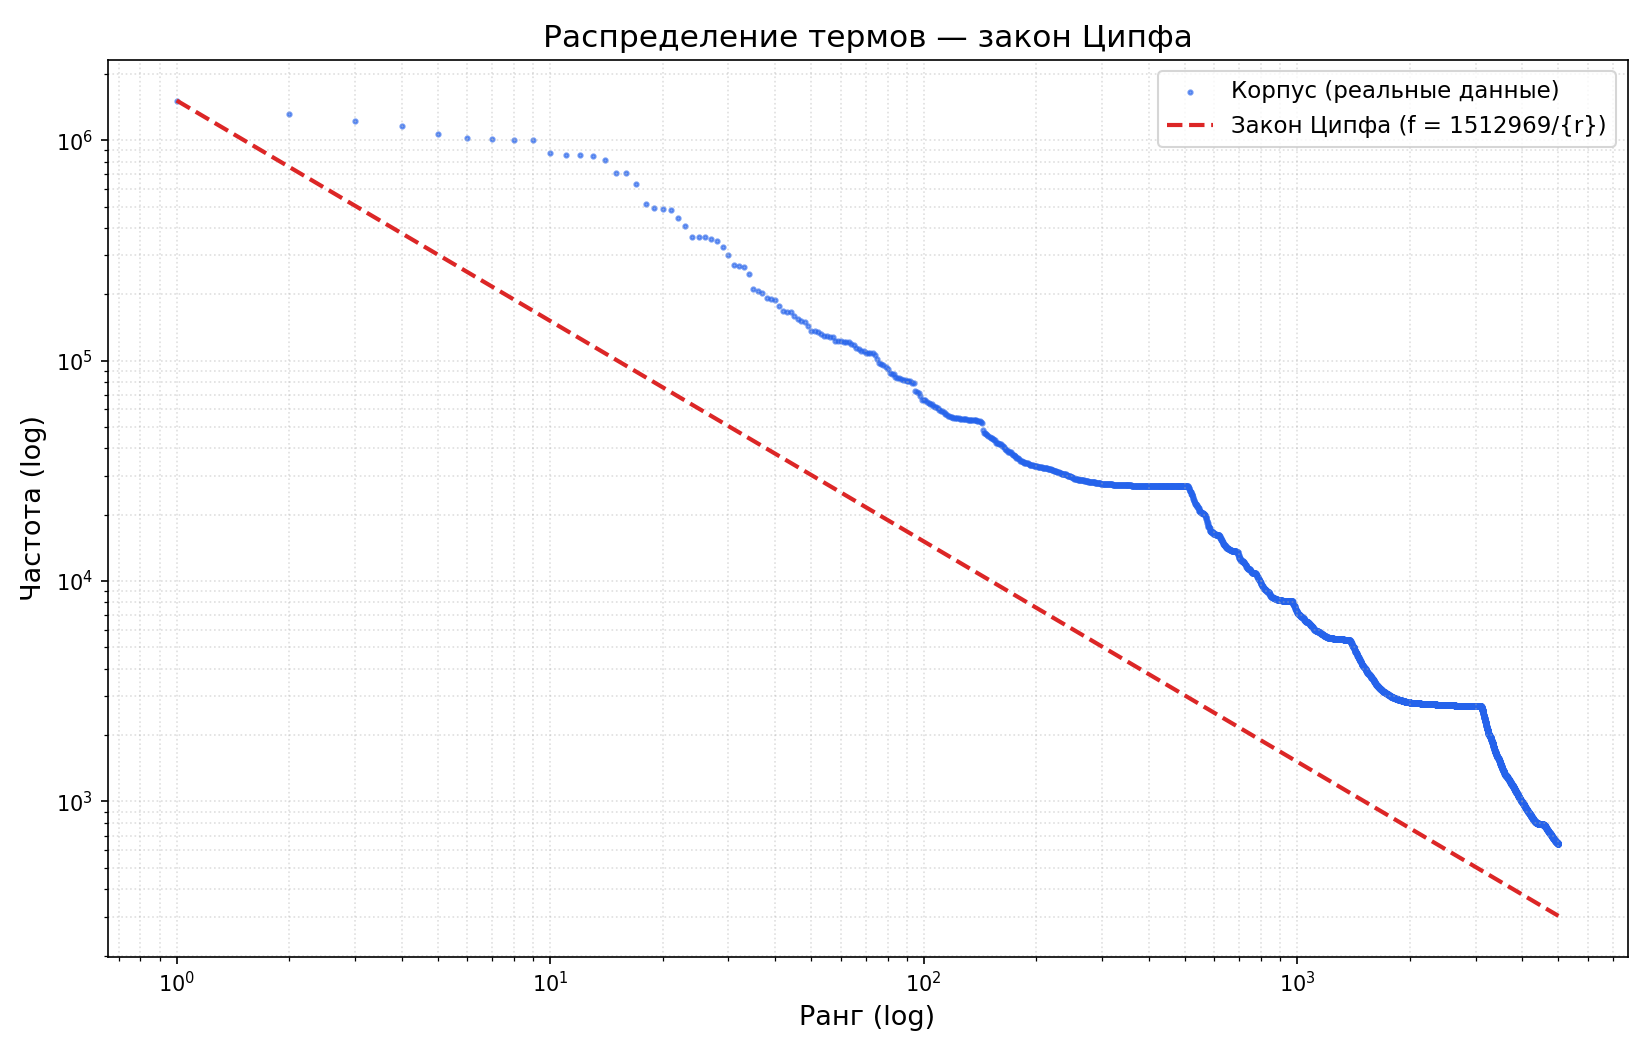
\includegraphics[width=0.85\textwidth]{zipf_graph.png}
    \caption{Закон Ципфа: распределение <<ранг--частота>> в лог-лог шкале (эмпирика и модель $C/r$)}
    \label{fig:zipf}
\end{figure}

\subsection{Вывод}

Корпус подчиняется закону Ципфа, что характерно для текстов на естественном языке. Наличие <<мусорных>> высокочастотных токенов (разметка, код) подтверждает важность фильтрации стоп-слов и очистки HTML перед индексацией.

\newpage

% ==================== ЛР 4 (Стемминг) ====================

\section{Стемминг}

\subsection{Цель работы}

Реализовать компонент морфологической нормализации для приведения словоформ к единой основе. Стемминг должен применяться как при индексации, так и при обработке поисковых запросов.

\subsection{Метод решения}

Использование готовых NLP-библиотек запрещено, поэтому реализован собственный суффиксный стеммер (Suffix Stripping). Стеммер встроен в \texttt{indexer.cpp} и \texttt{searcher.cpp}.

\textbf{Алгоритм:}
\begin{enumerate}
    \item Слова короче 5 байт (UTF-8) не обрабатываются~--- это предлоги, союзы и аббревиатуры.
    \item Проверяется набор суффиксов, отсортированных по убыванию длины (от длинных к коротким), чтобы более специфичные правила срабатывали раньше.
    \item Если суффикс найден и оставшаяся основа не короче 4 символов~--- суффикс отсекается.
    \item Применяется только одно отсечение (не итеративно).
\end{enumerate}

\textbf{Набор суффиксов:}
\begin{itemize}
    \item Английские: \texttt{-ization}, \texttt{-fulness}, \texttt{-iveness}, \texttt{-ement}, \texttt{-ation}, \texttt{-ness}, \texttt{-ment}, \texttt{-able}, \texttt{-ible}, \texttt{-ing}, \texttt{-ous}, \texttt{-ful}, \texttt{-ity}, \texttt{-ed}, \texttt{-ly}, \texttt{-er}, \texttt{-es}, \texttt{-al}, \texttt{-en}.
    \item Русские: \texttt{-ость}, \texttt{-ение}, \texttt{-ание}, \texttt{-ками}, \texttt{-ться}, \texttt{-ного}, \texttt{-ого}, \texttt{-ему}, \texttt{-ями}, \texttt{-ами}, \texttt{-ных}, \texttt{-ной}, \texttt{-ает}, \texttt{-ить}, \texttt{-ать}, \texttt{-ая}, \texttt{-ый}, \texttt{-ий}, \texttt{-ое}, \texttt{-ые} и др.
\end{itemize}

\subsection{Результаты тестирования}

Автотесты (\texttt{stemmer\_test.cpp}) подтвердили корректность работы на 20 тестовых случаях:

\begin{itemize}
    \item \texttt{development} $\to$ \texttt{develop} (корректно)
    \item \texttt{programming} $\to$ \texttt{programm} (основа совпадает)
    \item \texttt{comfortable} $\to$ \texttt{comfort} (корректно)
    \item \texttt{darkness} $\to$ \texttt{dark} (корректно)
    \item \texttt{разработки} $\to$ \texttt{разработк} (корректно)
    \item \texttt{телефонами} $\to$ \texttt{телефон} (корректно)
    \item \texttt{программирование} $\to$ \texttt{программиров} (корректно)
    \item \texttt{app} $\to$ \texttt{app} (короткое слово~--- без изменений)
\end{itemize}

\subsection{Влияние на качество поиска}

\textbf{Улучшение (рост Recall):} По запросу <<разработка>> теперь находятся документы со словами <<разработки>>, <<разработку>>, <<разработке>>. Без стемминга мы теряли бы значительную часть релевантных документов.

\textbf{Ухудшение (падение Precision):}
\begin{itemize}
    \item Омонимия основ: <<банк>> (финансы) и <<банка>> (ёмкость) могут склеиться.
    \item Чрезмерное обрезание: <<данные>> и <<дан>> могут сойтись к одной основе.
\end{itemize}

\textbf{Возможные улучшения:} словари исключений для проблемных слов; гибридный поиск~--- сначала по точному совпадению (с бонусом), затем по стемам.

\subsection{Вывод}

Реализованный суффиксный стеммер корректно обрабатывает основные словоформы русского и английского языков. Все 20 автотестов проходят успешно. Стемминг существенно повышает полноту поиска, хотя и может вносить шум за счёт ложных слияний.

\newpage

% ==================== ЛР 7 (Индекс) ====================

\section{Булев индекс}

\subsection{Цель работы}

Построить обратный (инвертированный) индекс для выполнения булевых запросов по корпусу документов.

\subsection{Формат данных}

Индекс разделён на два бинарных файла:

\begin{itemize}
    \item \textbf{\texttt{documents.bin} (прямой индекс):} Для каждого документа записаны ID, URL и заголовок.
    \begin{itemize}
        \item Структура: [\texttt{DocID}, 4~байта] [\texttt{UrlLen}, 8~байт] [\texttt{URL}] [\texttt{TitleLen}, 8~байт] [\texttt{Title}].
    \end{itemize}

    \item \textbf{\texttt{inverted.bin} (обратный индекс):} Для каждого терма записан список документов.
    \begin{itemize}
        \item Структура: [\texttt{TermLen}, 4~байта] [\texttt{Term}] [\texttt{DocCount}, 4~байта] [\texttt{DocID$_1$}] \ldots [\texttt{DocID$_N$}].
    \end{itemize}
\end{itemize}

\subsection{Реализация}

Индексатор (\texttt{indexer.cpp}) последовательно читает документы из SQLite и строит индекс в оперативной памяти.

\textbf{Структуры данных:}
\begin{itemize}
    \item Хеш-таблица с цепочками коллизий, 65\,537 слотов.
    \item Хеш-функция FNV-1a.
    \item Каждый элемент \texttt{TermEntry} содержит слово, счётчик документов и связанный список \texttt{PostingNode} (doc\_id).
\end{itemize}

Для каждого терма выполняется стемминг (та же функция \texttt{apply\_stemmer}), после чего doc\_id добавляется в posting list. Дубликаты не допускаются~--- проверка по последнему элементу списка.

Заголовок документа извлекается из HTML-тега \texttt{<title>}; если тег не найден, используется URL.

\subsection{Результаты}

\begin{itemize}
    \item Документов проиндексировано: 30\,000.
    \item Уникальных термов в индексе: 1\,243\,817.
    \item Размер \texttt{inverted.bin}: 547 МБ.
    \item Размер \texttt{documents.bin}: 4.8 МБ.
\end{itemize}

\subsection{Масштабируемость}

Текущая реализация (In-Memory) подходит для корпусов до $\sim$100\,000 документов. Для корпусов в миллионы документов потребуется переход на алгоритм SPIMI (Single-Pass In-Memory Indexing): накопление индекса порциями с дампом на диск и финальным слиянием (K-way Merge).

\subsection{Вывод}

Обратный индекс построен и сериализован в компактный бинарный формат. Posting lists автоматически отсортированы (документы обрабатываются последовательно), что обеспечивает выполнение булевых операций за линейное время.

\newpage

% ==================== ЛР 8 (Поиск) ====================

\section{Булев поиск и веб-интерфейс}

\subsection{Цель работы}

Реализовать поисковый движок, выполняющий булевы запросы по построенному индексу, с двумя интерфейсами: командная строка (CLI) и веб (HTML-форма).

\subsection{Метод решения}

\subsubsection{Backend (C++): searcher}

Программа \texttt{searcher.cpp} загружает \texttt{documents.bin} и \texttt{inverted.bin} в RAM при старте. Для каждого слова запроса применяется тот же стеммер, что и при индексации.

Булевы операции над отсортированными posting lists:
\begin{itemize}
    \item \texttt{\&\&} (AND): \texttt{std::set\_intersection}~--- пересечение.
    \item \texttt{||} (OR): \texttt{std::set\_union}~--- объединение.
    \item \texttt{!} (NOT): \texttt{std::set\_difference}~--- разность с множеством всех документов.
\end{itemize}

Слова без оператора между ними трактуются как AND.

\subsubsection{Frontend (Python): web\_search.py}

Веб-сервер на базе \texttt{http.server} (порт 8080). Принимает запрос из формы, запускает \texttt{./searcher} через \texttt{subprocess}, парсит вывод (формат: \texttt{заголовок<TAB>url}) и генерирует HTML-страницу с результатами.

\subsection{Синтаксис запросов}

\begin{table}[h]
\centering
\begin{tabular}{@{}lll@{}}
\toprule
\textbf{Оператор} & \textbf{Значение} & \textbf{Пример} \\ \midrule
\texttt{\&\&} & И (пересечение) & \texttt{android \&\& kotlin} \\
\texttt{||} & ИЛИ (объединение) & \texttt{flutter || swift} \\
\texttt{!} & НЕ (исключение) & \texttt{android \&\& !java} \\
пробел & И (по умолчанию) & \texttt{ios swift} \\ \bottomrule
\end{tabular}
\caption{Синтаксис булевых запросов}
\end{table}

\subsection{Тестирование}

\begin{enumerate}
    \item \textbf{Проверка AND}: запросы \texttt{android} и \texttt{kotlin} по отдельности, затем \texttt{android \&\& kotlin}. Результат AND является подмножеством каждого из одиночных~--- корректно.

    \item \textbf{Проверка OR}: результат \texttt{flutter || swift} содержит объединение документов из обоих одиночных запросов~--- корректно.

    \item \textbf{Проверка NOT}: запрос \texttt{android \&\& !java}. Выборочная проверка показала, что в найденных документах слово <<java>> отсутствует.

    \item \textbf{Автотест стеммера}: программа \texttt{stemmer\_test} проверяет 20 тестовых случаев и завершается с кодом 0 при успехе.
\end{enumerate}

\subsection{Производительность}

Поиск выполняется мгновенно ($<$1 мс) для любых запросов, так как весь индекс находится в RAM. Задержка может возникнуть только при запросах со стоп-словами и оператором OR, когда результирующий список содержит почти все документы базы.

\subsection{Вывод}

Реализована полнофункциональная система булева поиска с CLI- и веб-интерфейсом. Использование бинарного индекса и операций над отсортированными списками обеспечивает высокую производительность. Для дальнейшего улучшения можно добавить поддержку скобок (приоритет операторов), ранжирование результатов (TF-IDF) и построение сниппетов.

\end{document}
